\section{Course Introduction}

The concepts and techniques in this course are probably the most useful in engineering. A {\it signal} is a function of one or more independent variables conveying information about a physical (or virtual) phenomena. A {\it system} may respond to signals to produce other signals, or produce signals directly.

  \begin{center}
    \begin{tikzpicture}[auto, node distance=3cm,>=latex']
      \node [input, name=input] {};
      \node [block, right of=input] (system) {System $T$};
      \node [output, right of=system] (output) {};

      \draw [draw,->] (input) -- node {Input $x$} (system);
      \draw [->] (system) -- node {Output $y$} (output);
    \end{tikzpicture}
  \end{center}

  This course is about the mathematical models and related techniques for the design and understanding of systems as signal transformations. We focus on a broadly useful class of systems, known as {\it linear, time-invariant systems}. You will learn about:

  \begin{itemize}
  \item the representation and analysis of signals as information carrying channels
  \item and how to analyze and implement linear, time-invariant systems to transform those signals.
  \end{itemize}
  
  Example: Electrical Circuits\\
  
  This is a Sallen-Key filter, a second-order system commonly use to select frequencies from a signal:

  \begin{circuitikz}[american voltages,scale=0.8, every node/.style={transform shape}]
\draw
(7,3.5) node[op amp] (opamp1) {}
(0,4) to[R,l=$R_1$,o-] (2,4)
(2,4) to[short] (2,5)
(2,5) to[C,l=$C_1$] (8.2,5)
(8.2,5) to[short] (opamp1.out) 
(2,4) to[R, l=$R_2$] (4,4)
(4,4) to[C, l=$C_2$] (4,0)
(0,0) to[short,o-o] (12,0)
(4,4) to[short] (opamp1.-)
(opamp1.+) to[short] (5.8,1.75)
(5.8,1.75) to[short] (8.2,1.75)
(opamp1.out) to[R, l=$(1-\beta)R$] (8.2,1.75)
(8.2,1.75) to[R, l=$\beta R$] (8.2,0)
(opamp1.out) to[short, -o] (12,3.5)
(0,4) to[open, v=$x(t)$] (0,0)
(12,3.5) to[open, v=$y(t)$] (12,0);
\end{circuitikz}

How do we choose the values of the resistors and capacitors to select the frequencies we are interested in? How do we determine what those frequencies are?

Example: Robotic Joint\\

  This is a Linear, Time-Invariant model of a DC motor, a mixture of electrical and mechanical components.
  
\tikzstyle{block} = [draw, fill=gray!20, rectangle, 
    minimum height=3em, minimum width=3em]
\tikzstyle{sum} = [draw, fill=gray!20, circle, node distance=1cm]
\tikzstyle{input} = [coordinate]
\tikzstyle{output} = [coordinate]
\tikzstyle{pinstyle} = [pin edge={to-,thin,black}]

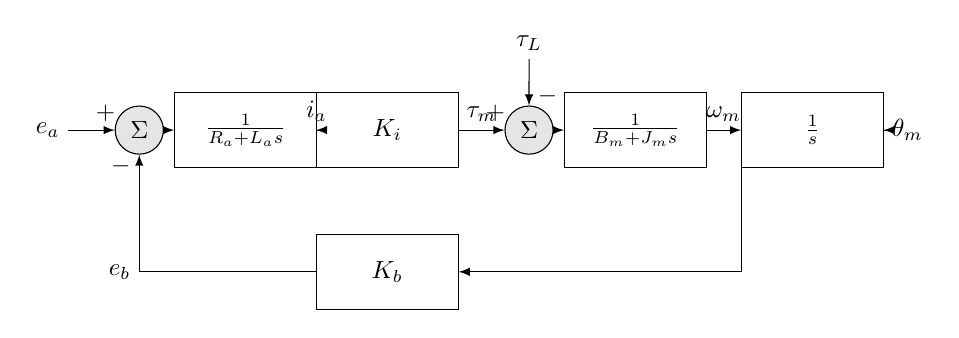
\begin{tikzpicture}[auto, node distance=2cm,>=latex, scale=0.9, every node/.style={transform shape}]

  \node [sum] at (2.5,0) (vsum) {$\Sigma$};
  \node [block] at (4,0) (arm) {$\frac{1}{R_a + L_a s}$};
  \node [block] at (6,0) (torque) {$K_i$};
  \node [sum] at (8,0) (tsum) {$\Sigma$};
  \node [block] at (9.5,0) (motor) {$\frac{1}{B_m + J_m s}$};
  \node [block] at (12,0) (int) {$\frac{1}{s}$};
  \node [block] at (6,-2) (backemf) {$K_b$};

  \draw [->] (1.5,0) node [left] {$e_a$} -- node[pos=0.8] {$+$} (vsum);
  \draw [->] (vsum) -- (arm);
  \draw [->] (arm) -- (torque) node [midway,above] {$i_a$};
  \draw [->] (torque) -- node[pos=0.8] {$+$} (tsum) node [midway,above] {$\tau_m$};
  \draw [->] (tsum) -- (motor);
  \draw [->] (8,1) node[above] {$\tau_L$} -- node[pos=0.8] {$-$} (tsum);
  \draw [->] (motor) -- (int) node [midway,above] {$\omega_m$};
  \draw [->] (11,0) |- (backemf);
  \draw [->] (backemf) -| node[midway] {$e_b$} node[pos=0.95] {$-$} (vsum);
  \draw [->] (int) -- (13,0) node[right] {$\theta_m$};
\end{tikzpicture}

How do we convert the motor into a servo for use in a robotic joint? What are its characteristics (e.g. how fast can it move)?

Example: Audio Processing\\

  Suppose you record an interview for a podcast, but during an important part of the discussion, the HVAC turns on and there is an annoying noise in the background.

\begin{center}

\includegraphics[scale=0.5]{figures/noisysignal.pdf}
\end{center}

  How could you remove the noise minimizing distortion to the rest of the audio?

  Example: Communications\\
  
  Consider a wireless sensor, that needs to transmit to a base station, e.g. a wireless mic system. 
  \begin{center}
  \tikzset{block/.style = {draw, fill=white, rectangle,
              minimum height=3em, minimum width=2cm},
    input/.style = {coordinate},
    output/.style = {coordinate},
    pinstyle/.style = {pin edge={to-,t,black}},
    radiation/.style={decorate,decoration={expanding waves,angle=12,segment length=4pt}}
  }
   \begin{tikzpicture}[auto, node distance=2cm,>=latex']
\node[block](tx){Sensor Node};
\node[antenna] at (tx.east) {};
\node[block,right = 5cm of tx](rx){Base Station};
\node[antenna,xscale=-1] at (rx.west) {};

\draw[radiation] ([shift={(1cm,2cm)}]tx.east)-- node [above=5mm] {} ([shift={(-1cm,2cm)}]rx.west);
\end{tikzpicture}
\end{center}

How should the signal be processed so it can be transmitted? How should the received signal be processed?

Applications of this material occur in all areas of science and engineering.

When we have a measured output but are unsure what combination of inputs and system components could have produced it, we have a {\it modeling} problem.

    \begin{center}
    \begin{tikzpicture}[auto, node distance=3cm,>=latex']
      \node [input, name=input] {};
      \node [block, right of=input] (system) {?};
      \node [output, right of=system] (output) {};

      \draw [draw,->] (input) -- node {Input ?} (system);
      \draw [->] (system) -- node {Output $y$} (output);
    \end{tikzpicture}
  \end{center}
  
   Models are the bedrock of the scientific method and are required to apply the concepts of this course to engineering problems. 

   When we know the input and the system description and desire to know the output we have an {\it analysis} problem. 

    \begin{center}
    \begin{tikzpicture}[auto, node distance=3cm,>=latex']
      \node [input, name=input] {};
      \node [block, right of=input] (system) {System $T$};
      \node [output, right of=system] (output) {};

      \draw [draw,->] (input) -- node {Input $x$} (system);
      \draw [->] (system) -- node {Output ?} (output);
    \end{tikzpicture}
  \end{center}
  
  Analysis problems are the kind you have encountered most often already. For example, given an electrical circuit and an applied voltage or current, what are the voltages and currents across and through the various components.

  When we know either the input and desired output and seek the system to perform this transformation,
  \begin{center}
    \begin{tikzpicture}[auto, node distance=3cm,>=latex']
      \node [input, name=input] {};
      \node [block, right of=input] (system) {System ?};
      \node [output, right of=system] (output) {};

      \draw [draw,->] (input) -- node {Input $x$} (system);
      \draw [->] (system) -- node {Output $y$} (output);
    \end{tikzpicture}
  \end{center}

  or we know the system description and output and desire the input that would generate the output,

    \begin{center}
    \begin{tikzpicture}[auto, node distance=3cm,>=latex']
      \node [input, name=input] {};
      \node [block, right of=input] (system) {System $T$};
      \node [output, right of=system] (output) {};

      \draw [draw,->] (input) -- node {Input ?} (system);
      \draw [->] (system) -- node {Output $y$} (output);
    \end{tikzpicture}
  \end{center}

  we have a {\it design problem}.
  
  This course focuses on modeling and analysis. Subsequent courses, e.g. ECE 3704, focus more on analysis and design.

  This course considers applications to electrical circuits and devices for measurement and control of the physical world and is broadly applicable to all ECE majors.

  Some Examples:
  
  \begin{itemize}
  \item Controls, Robotics, \& Autonomy: LTI systems theory forms the basis of perception and control of machines.
  \item Communications \& Networking: LTI systems theory forms the basis of transmission and reception of signals, e.g. AM and FM radio.
  \item Machine Learning: LTI systems are often used to pre-process samples or to create basis functions to improve learning.
  \item Energy \& Power Electronic Systems: linear circuits are often modeled as LTI systems.
  \end{itemize}

The learning objectives for the course are:

\begin{enumerate}
\item Describe a given system using a block-level description and identify the input/output signals.
\item Mathematically model continuous and discrete linear, time-invariant systems using differential and difference equations
  respectively.
\item Analyze the use of filters and their interpretation in the time and frequency domains and implement standard filters in
  hardware and/or software.
\item Apply computations of the four fundamental Fourier transforms to the analysis and design of linear systems.
\item Communicate solutions to problems and document projects within the domain of signals and systems through formal written documents.
\end{enumerate}

Tentative Schedule:\\

\begin{itemize}
\item Mathematical Representation of Signals and Systems
\item Linear, Time-Invariant Systems
\item Fourier Series
\item Fourier Transforms
\item Frequency Response and Filtering
\item Sampling and Reconstruction of Signals
\item Project
\end{itemize}

See the Canvas site for the up-to-date schedule.

Prerequisites: Math\\

\begin{itemize}
\item Algebra (real and complex)
\item Calculus
\item Discrete Math
\item Differential Equations
\end{itemize}

ECE 2024 is required for knowledge of continuous signals representation as voltages and currents, and the analysis and construction of circuits containing resistors, capacitors, inductors, and operational amplifiers

\begin{itemize}
\item $v = iR$\hspace{2em}
  \begin{circuitikz}[american voltages,scale=0.8, every node/.style={transform shape}]
    \draw
    (0,0) to[R,l=$R$] (4,0);
  \end{circuitikz}
  
\item $i = Cv^\prime$ \hspace{2em}
  \begin{circuitikz}[american voltages,scale=0.8, every node/.style={transform shape}]
    \draw
    (0,0) to[C,l=$C$] (4,0);
  \end{circuitikz}
\item $v = Li^\prime$ \hspace{2em}
  \begin{circuitikz}[american voltages,scale=0.8, every node/.style={transform shape}]
    \draw
    (0,0) to[L,l=$L$] (4,0);
  \end{circuitikz}
\item KVL
\item KCL
\item Ideal Op-Amp
\end{itemize}

ECE 2514 is required for the ability to model and simulate physical systems using computational tools, and basic programming ability.

\begin{itemize}
\item Matlab for general computation and plotting
\item C++ (a small subset) for implementing digital filters
\end{itemize}

ECE 2544 is required for for knowledge of digital signal representation and the analysis and construction of circuits containing combinatorial and sequential logic.

Textbook:\\
  Oppenheim, A. V., Willsky, A. S., and Nawab, S. H. Signals and Systems. ii, Essex UK: Prentice Hall Pearson, 1996.\\

  This is an older, but very good book. However there are many, many texts that cover the same material. {\bf Engaged} reading the textbook is one of the most important things you can do to learn this material.

  Note, these notes should not be considered a replacement for the textbook.

